%%%%%%%%%%%%%%%%
\section{Introduction}

\subsection{}
\begin{frame}{Introduction}{}
    \begin{figure}[H]
        \centering
        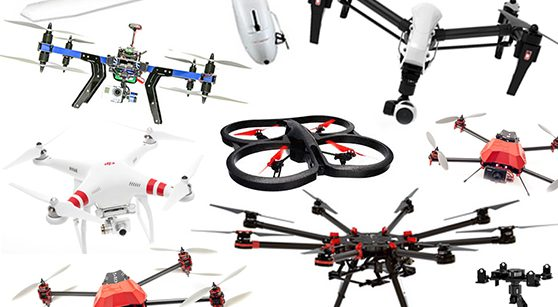
\includegraphics[width=.6\linewidth]{figures/multicopters}
    \end{figure}
    \begin{itemize}
         \item Surveillance and inspection
         \item Rescue
         \item Aerial photography
         \item ...
    \end{itemize}

\end{frame}

\begin{frame}{Introduction}{Prototype}
    \begin{figure}[H]
        \centering
        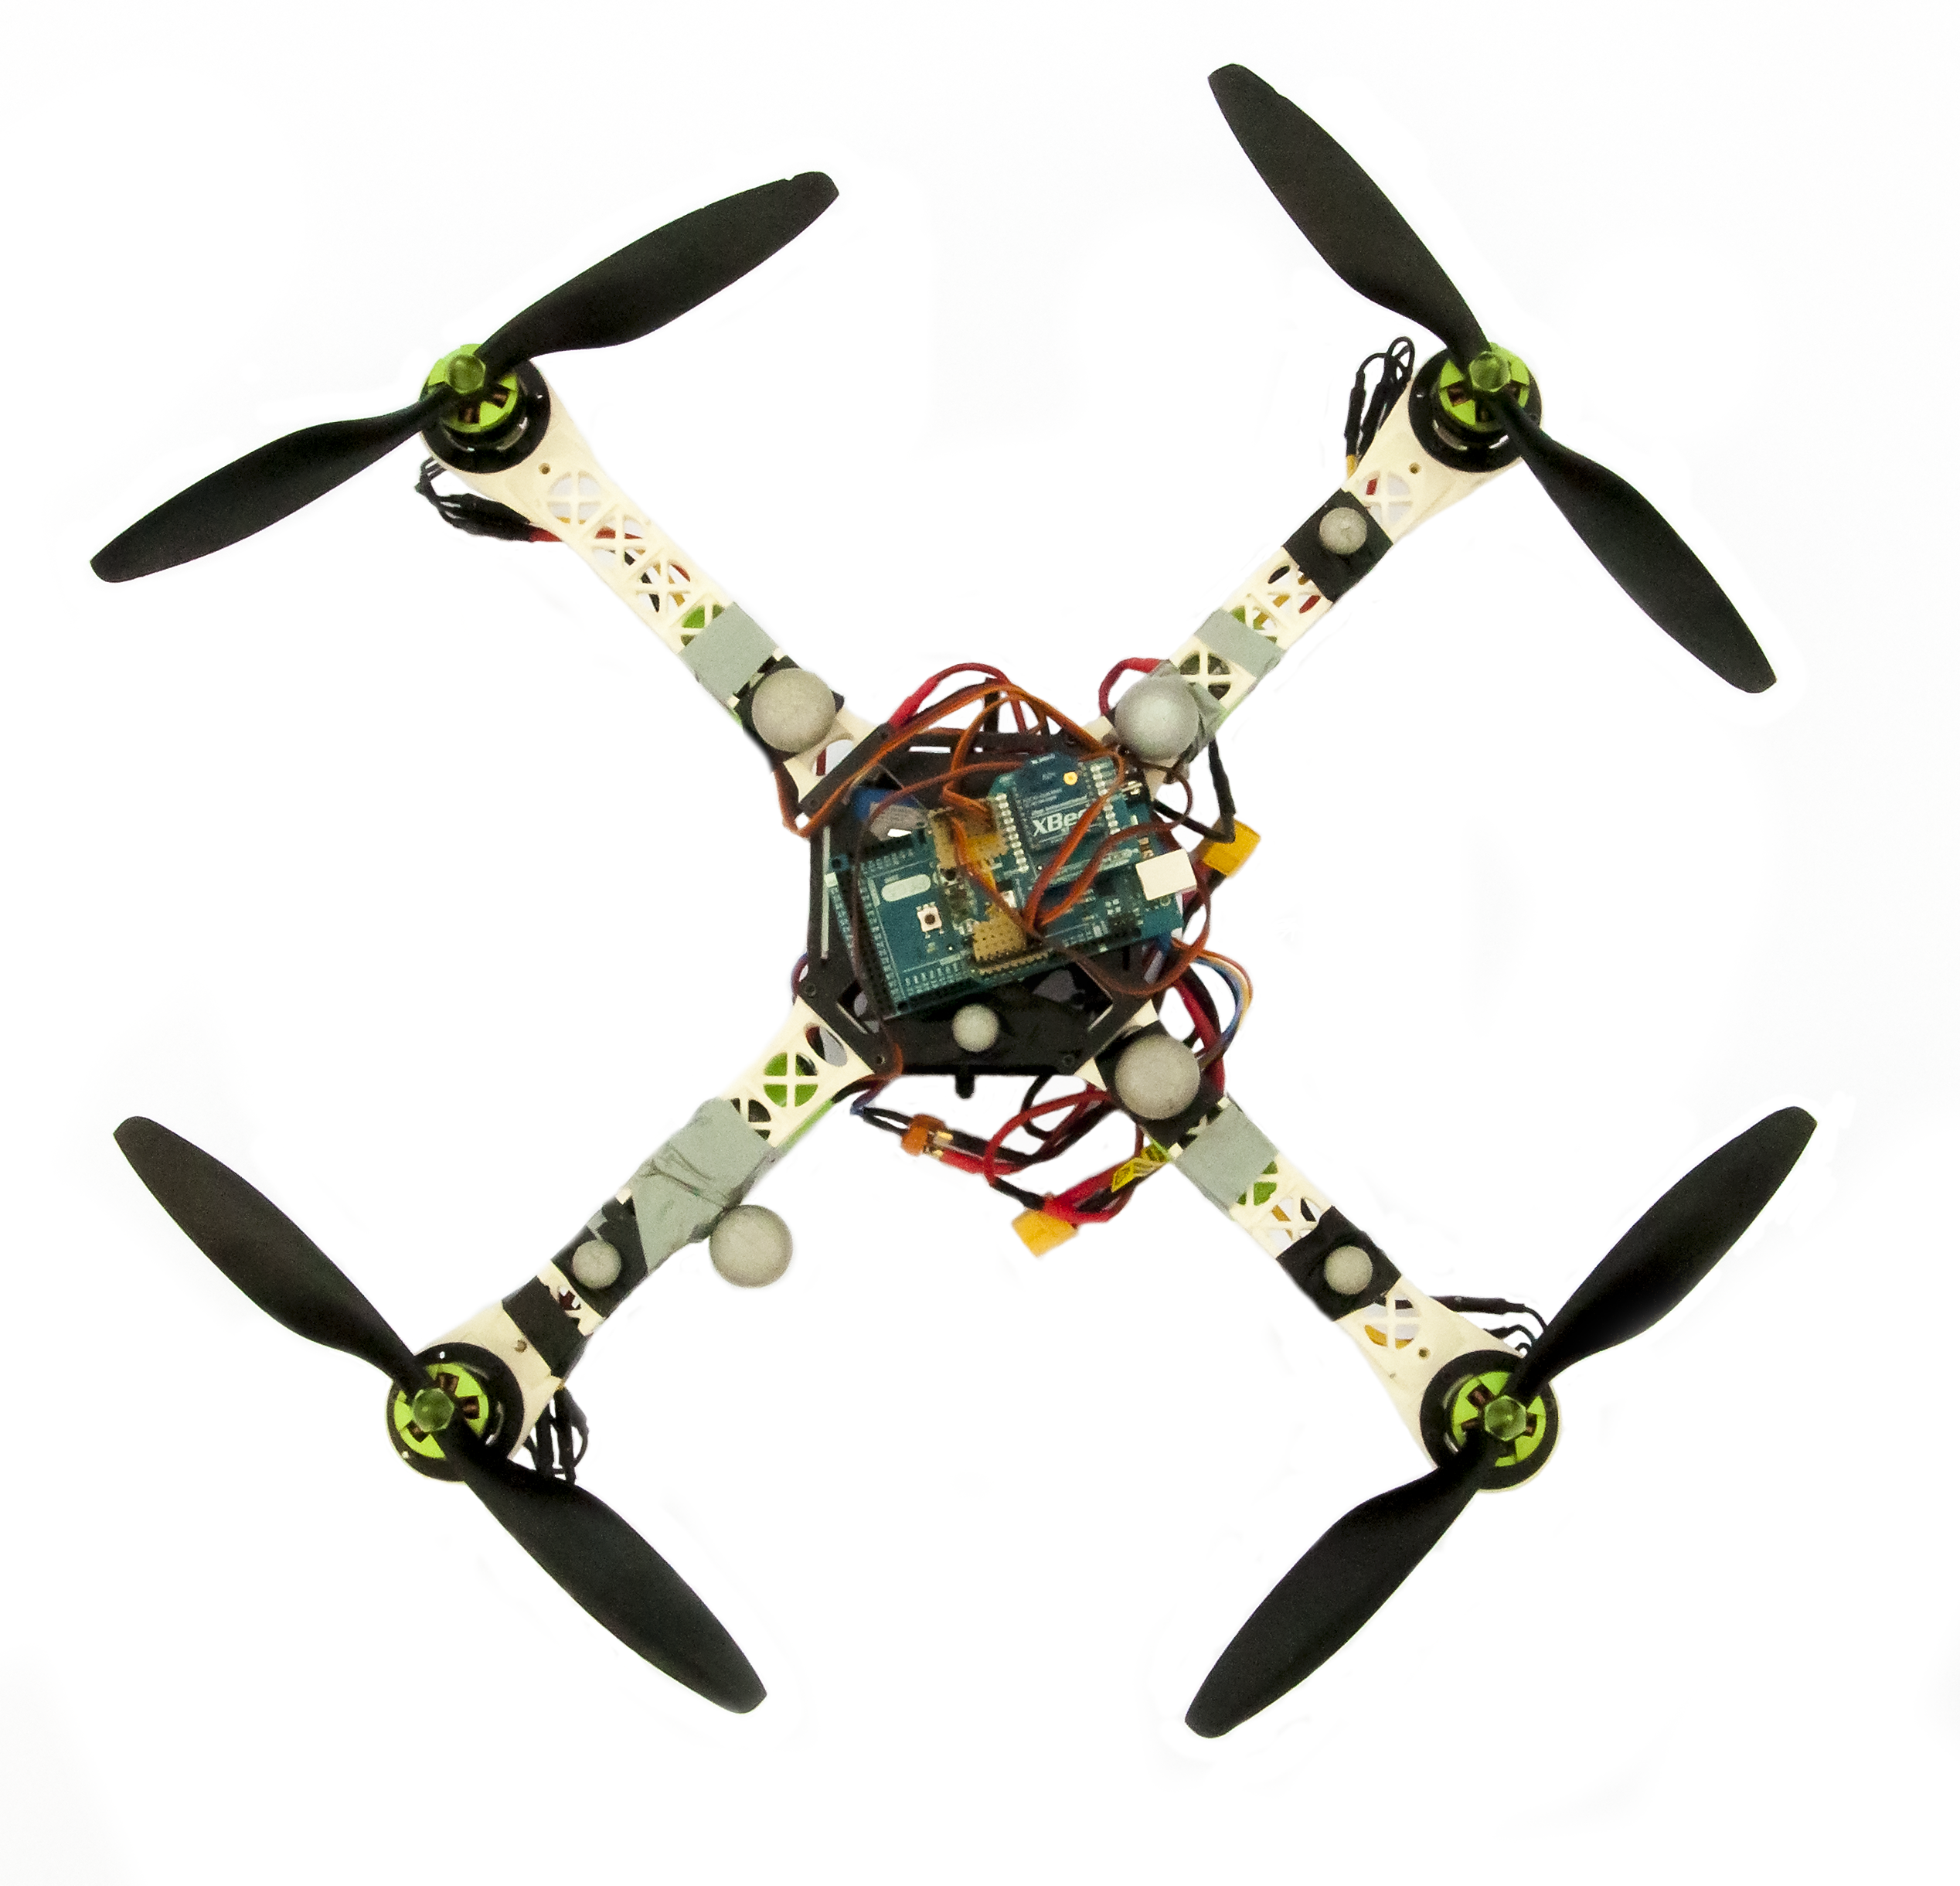
\includegraphics[width=.45\linewidth]{figures/quadcopter}
    \end{figure}
    \begin{itemize}
        \item 
       \end{itemize}     
\end{frame}

%%%%%%%%%%%%%%%%
\section{Model}
\subsection{Attitude Model}
\begin{frame}{Model}{Attitude Model}
    \only<1>{
        \begin{figure}[H]
            \includegraphics[width=0.6\textwidth]{figures/dronediagram1}
        \end{figure}            
    }
    \only<2>{
        \begin{figure}[H]
            \includegraphics[width=0.6\textwidth]{figures/dronediagram2}
        \end{figure}            
    }
    \only<3>{
        \begin{figure}[H]
            \includegraphics[width=0.6\textwidth]{figures/dronediagram3}
        \end{figure}            
    }
    \only<4>{
        \begin{figure}[H]
            \includegraphics[width=0.6\textwidth]{figures/dronediagram4}
        \end{figure}            
    }
    \only<5>{
        \begin{figure}[H]
            \includegraphics[width=0.6\textwidth]{figures/dronediagram5}
        \end{figure}            
    }
    \only<6>{
        \begin{figure}[H]
            \includegraphics[width=0.6\textwidth]{figures/dronediagram6}
        \end{figure}            
    }
    \only<7>{
        \begin{figure}[H]
            \includegraphics[width=0.6\textwidth]{figures/dronediagram7}
        \end{figure}            
    }
    \only<8>{
        \begin{figure}[H]
            \includegraphics[width=0.6\textwidth]{figures/dronediagram8}
        \end{figure}            
    }   
\end{frame}

\begin{frame}{Model}{Attitude Model}
     \begin{itemize}
         \item Dynamic Equations
        \end{itemize}
    \uncover<2-4>{            
    \begin{flalign}
    J \alpha=\sum\tau \nonumber
    \end{flalign}
    }
    \uncover<3-4>{
        \begin{align}
        J_x \ddot{\phi}&=(F_4-F_2) L \nonumber \\
        J_y \ddot{\theta}&=(F_1-F_3) L \nonumber \\
        J_z \ddot{\psi}&=\tau_1-\tau_2+\tau_3-\tau_4 \nonumber
        \end{align}
    }
        \uncover<4>{
        \begin{align}
        J_x \ddot{\phi}&=k_\mathrm{th} (\omega^2_4-\omega^2_2)  L \nonumber\\
        J_y \ddot{\theta}&=k_\mathrm{th} (\omega^2_1-\omega^2_3)  L \nonumber\\
        J_z \ddot{\psi}&=k_\mathrm{d} (\omega^2_1-\omega^2_2+\omega^2_3-\omega^2_4) \nonumber
        \end{align}
        }    
    
\end{frame}

%%
% TOC
\begin{frame}{Agenda}{}
    \tableofcontents
\end{frame}

%%